\section{Experimental Setup1}
\label{expSetup}
The experimental setup that is described in this section, is designed to measure, the properties of LXe scintillation. 
However it is designed in a modular way, so it can serve different requirements from different future experiments. 
There are three main building blocks consisting the full setup, The purification and circulation system, the cryogenic system, 
and the detector system. Each building block can be replaced without effecting the others, this concept as well as some design 
ideas were taken from~\cite{Giboni}. The full assembly (figure.~\ref{fig:fulldet}) is held on three separate wracks, one for the DAQ, 
while the two others which hold the the detector and purification system are joined using a 100mm bar with shock absorbers on both sides.   

\begin{figure}[t!]
\centerline{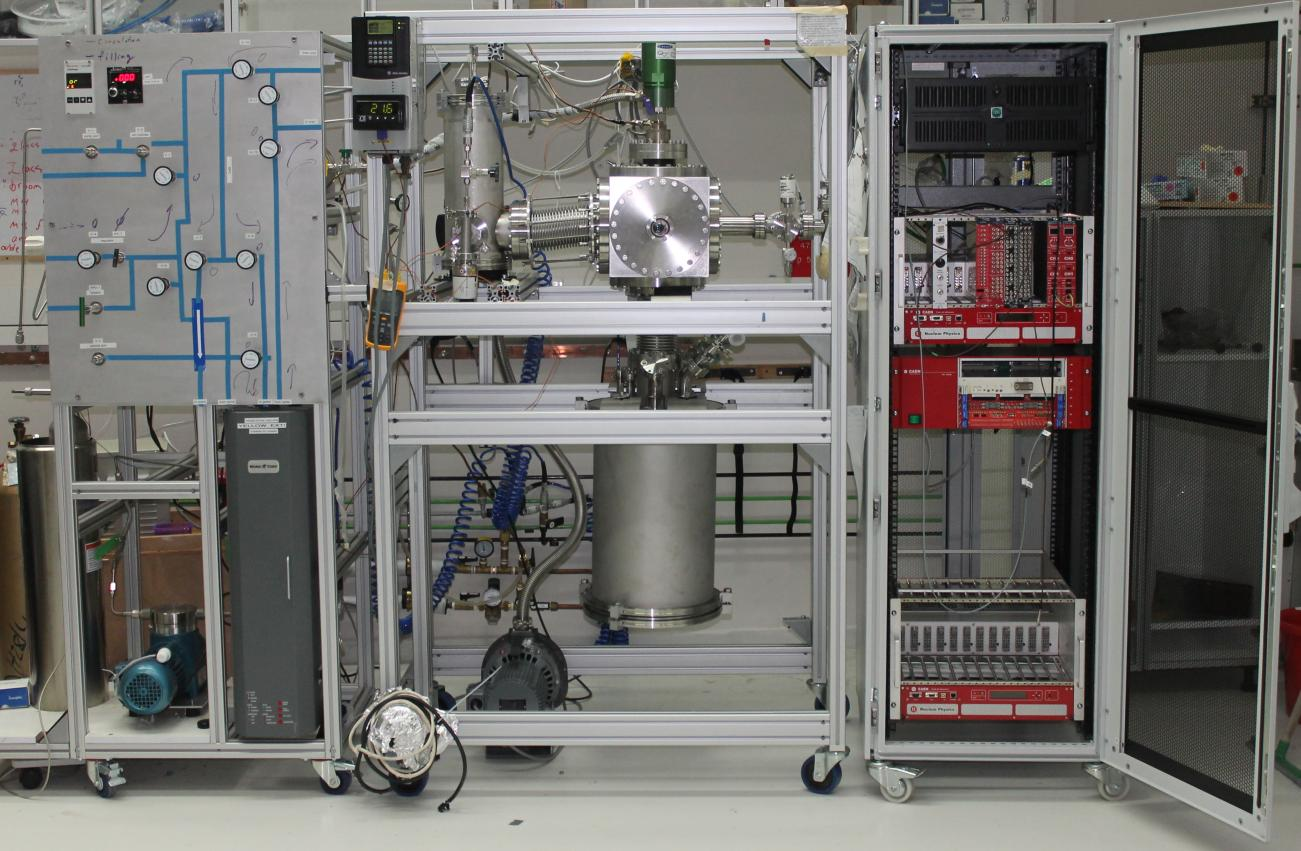
\includegraphics[width=1.\linewidth]{FullDet.jpg}}
\caption{Direxeno. On the left the purification system, in the middle the cryogenic and detector chamber, and on th right the Data acquisition system.}
\label{fig:fulldet}
\end{figure}

\subsection{Gas handling system \mmd{Can we write Gas Purification system instead?}}
\label{subsec:gas}

A typical LXe detector must keep a high level of purity. Careful selection and meticulously cleaning of all parts before mounting, is needed, however is not sufficient. The desired level in most detectors of impurity concentration is at the level of 1 ppb $O_2$ equivalent~\cite{Aprile:2009dv}. This is crucial to allow ionization electrons drift for several cm. To reach that level in a reasonable amount of time (several days instead of months), continuous purification is needed. The gas system, provides this process, alongside with all gas handling operations such as filling and recuperation.

During purification mode, xenon is taken from the chamber (in liquid phase)
passes through a heat exchanger\footnote{GEA GBS100M-24 plate heat exchanger} where it is heated and vapored. Then the xenon is forced by a KNF diaphragm pump into a hot getter\footnote{MONO-TORR
PS4-MT15-R-2} which cleans the xenon from most impurities. The xenon
also passes through an MKS Mass Flow Controller\footnote{MKS mass flow controller} (MFC) which enables the monitoring of heat load. 

After the xenon is purified, it is delivered back to the cryogenic system through the heat exchanger, there most of the  xenon gas is liquefied before it continuous back to the chamber. A schematic of this system is shown in fig.~\ref{fig:gasSchematic}.


\begin{figure}[t!]
\centerline{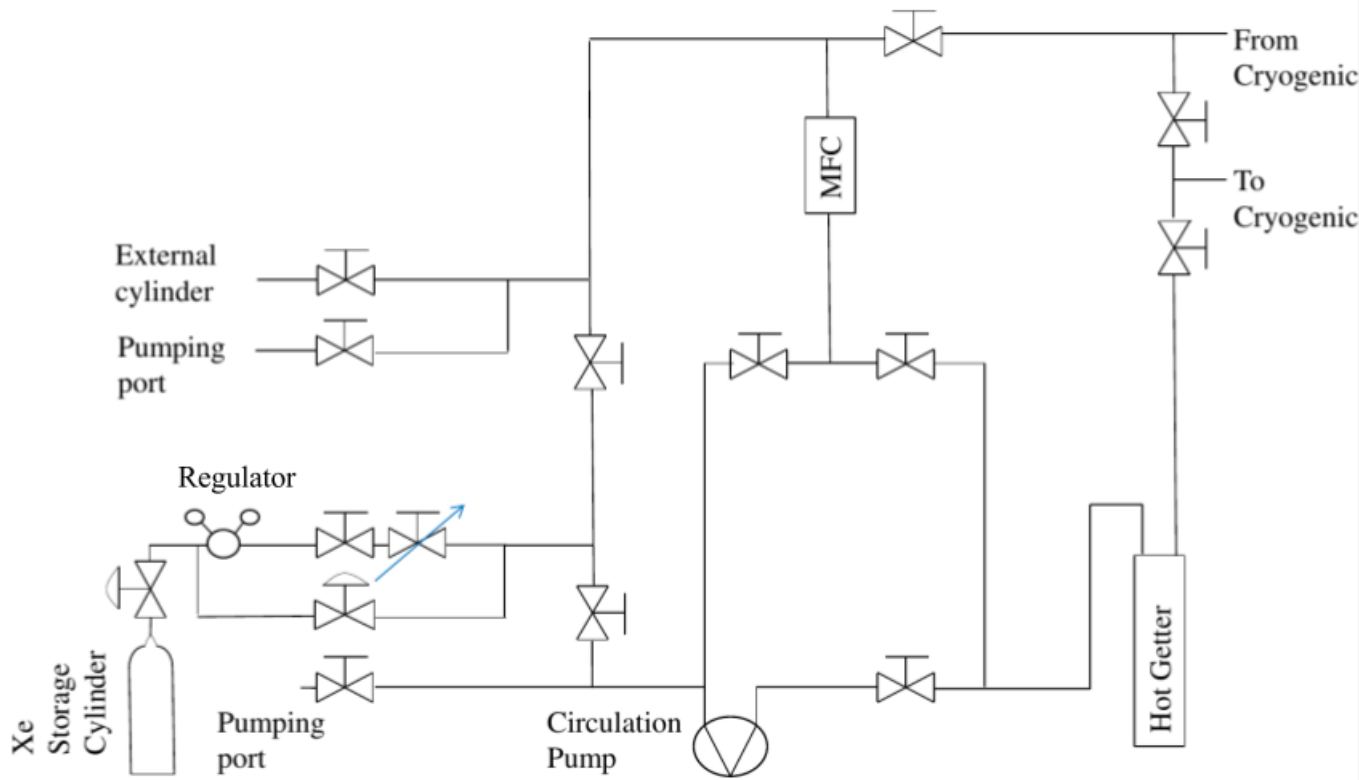
\includegraphics[width=1.\linewidth]{GasSchematics.png}}
\caption{Schematics of the purification system. High pressure valves are indicated as valves with arcs. Needle valves are indicated as a valve with an arrow.}
\label{fig:gasSchematic}
\end{figure}
\subsection{Cryogenic System}
\label{subsec:cryo}

Remote cooling is generally used in DM experiments due to background radiating from the cooler to the detector. Although in our system this is not of great importance there are still several advantages to remote cooling such as: lowering acoustic noise from the cryo-cooler and flexibility to design changes. The cryogenic system is connected on one side to the gas system and on the other to the detector chamber, any change in the system (e.g, cooler type or model) requires the change of that specific part without changing the detector nor the gas system.

The system is made out of two chambers, the outer vessel (OV) which holds the insulation vacuum, and the inner vessel (IV) which holds the xenon. In addition to the vacuum which prevents heat leaks from diffusion and convection, the entire IV is covered by multi layer aluminized Myler to prevent heating via radiation. A picture of the detector and the CAD design are shown in Fig~\ref{fig:cryo}. 
\begin{figure}
   \centering
    \begin{subfigure}[b]{0.25\textheight}
    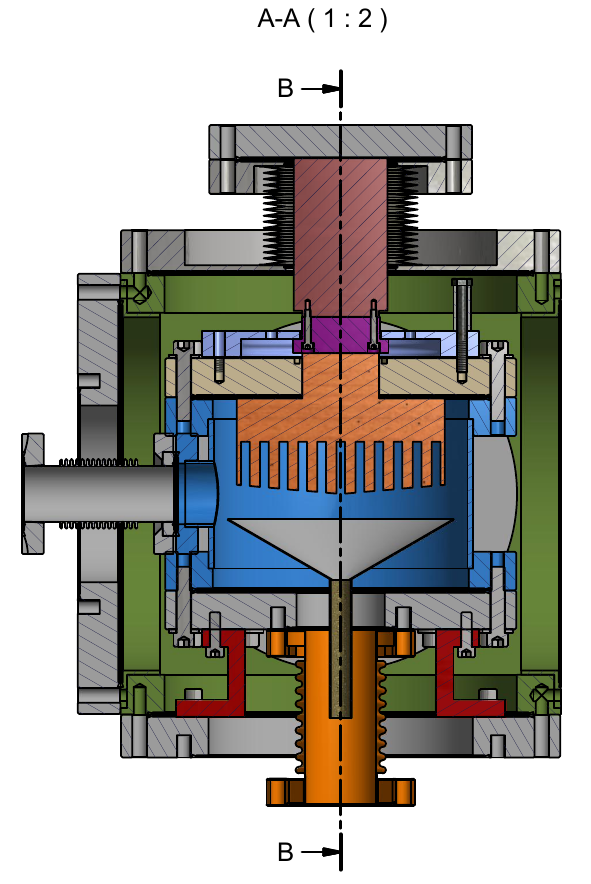
\includegraphics[width=\textwidth]{cryogenic1.png}
    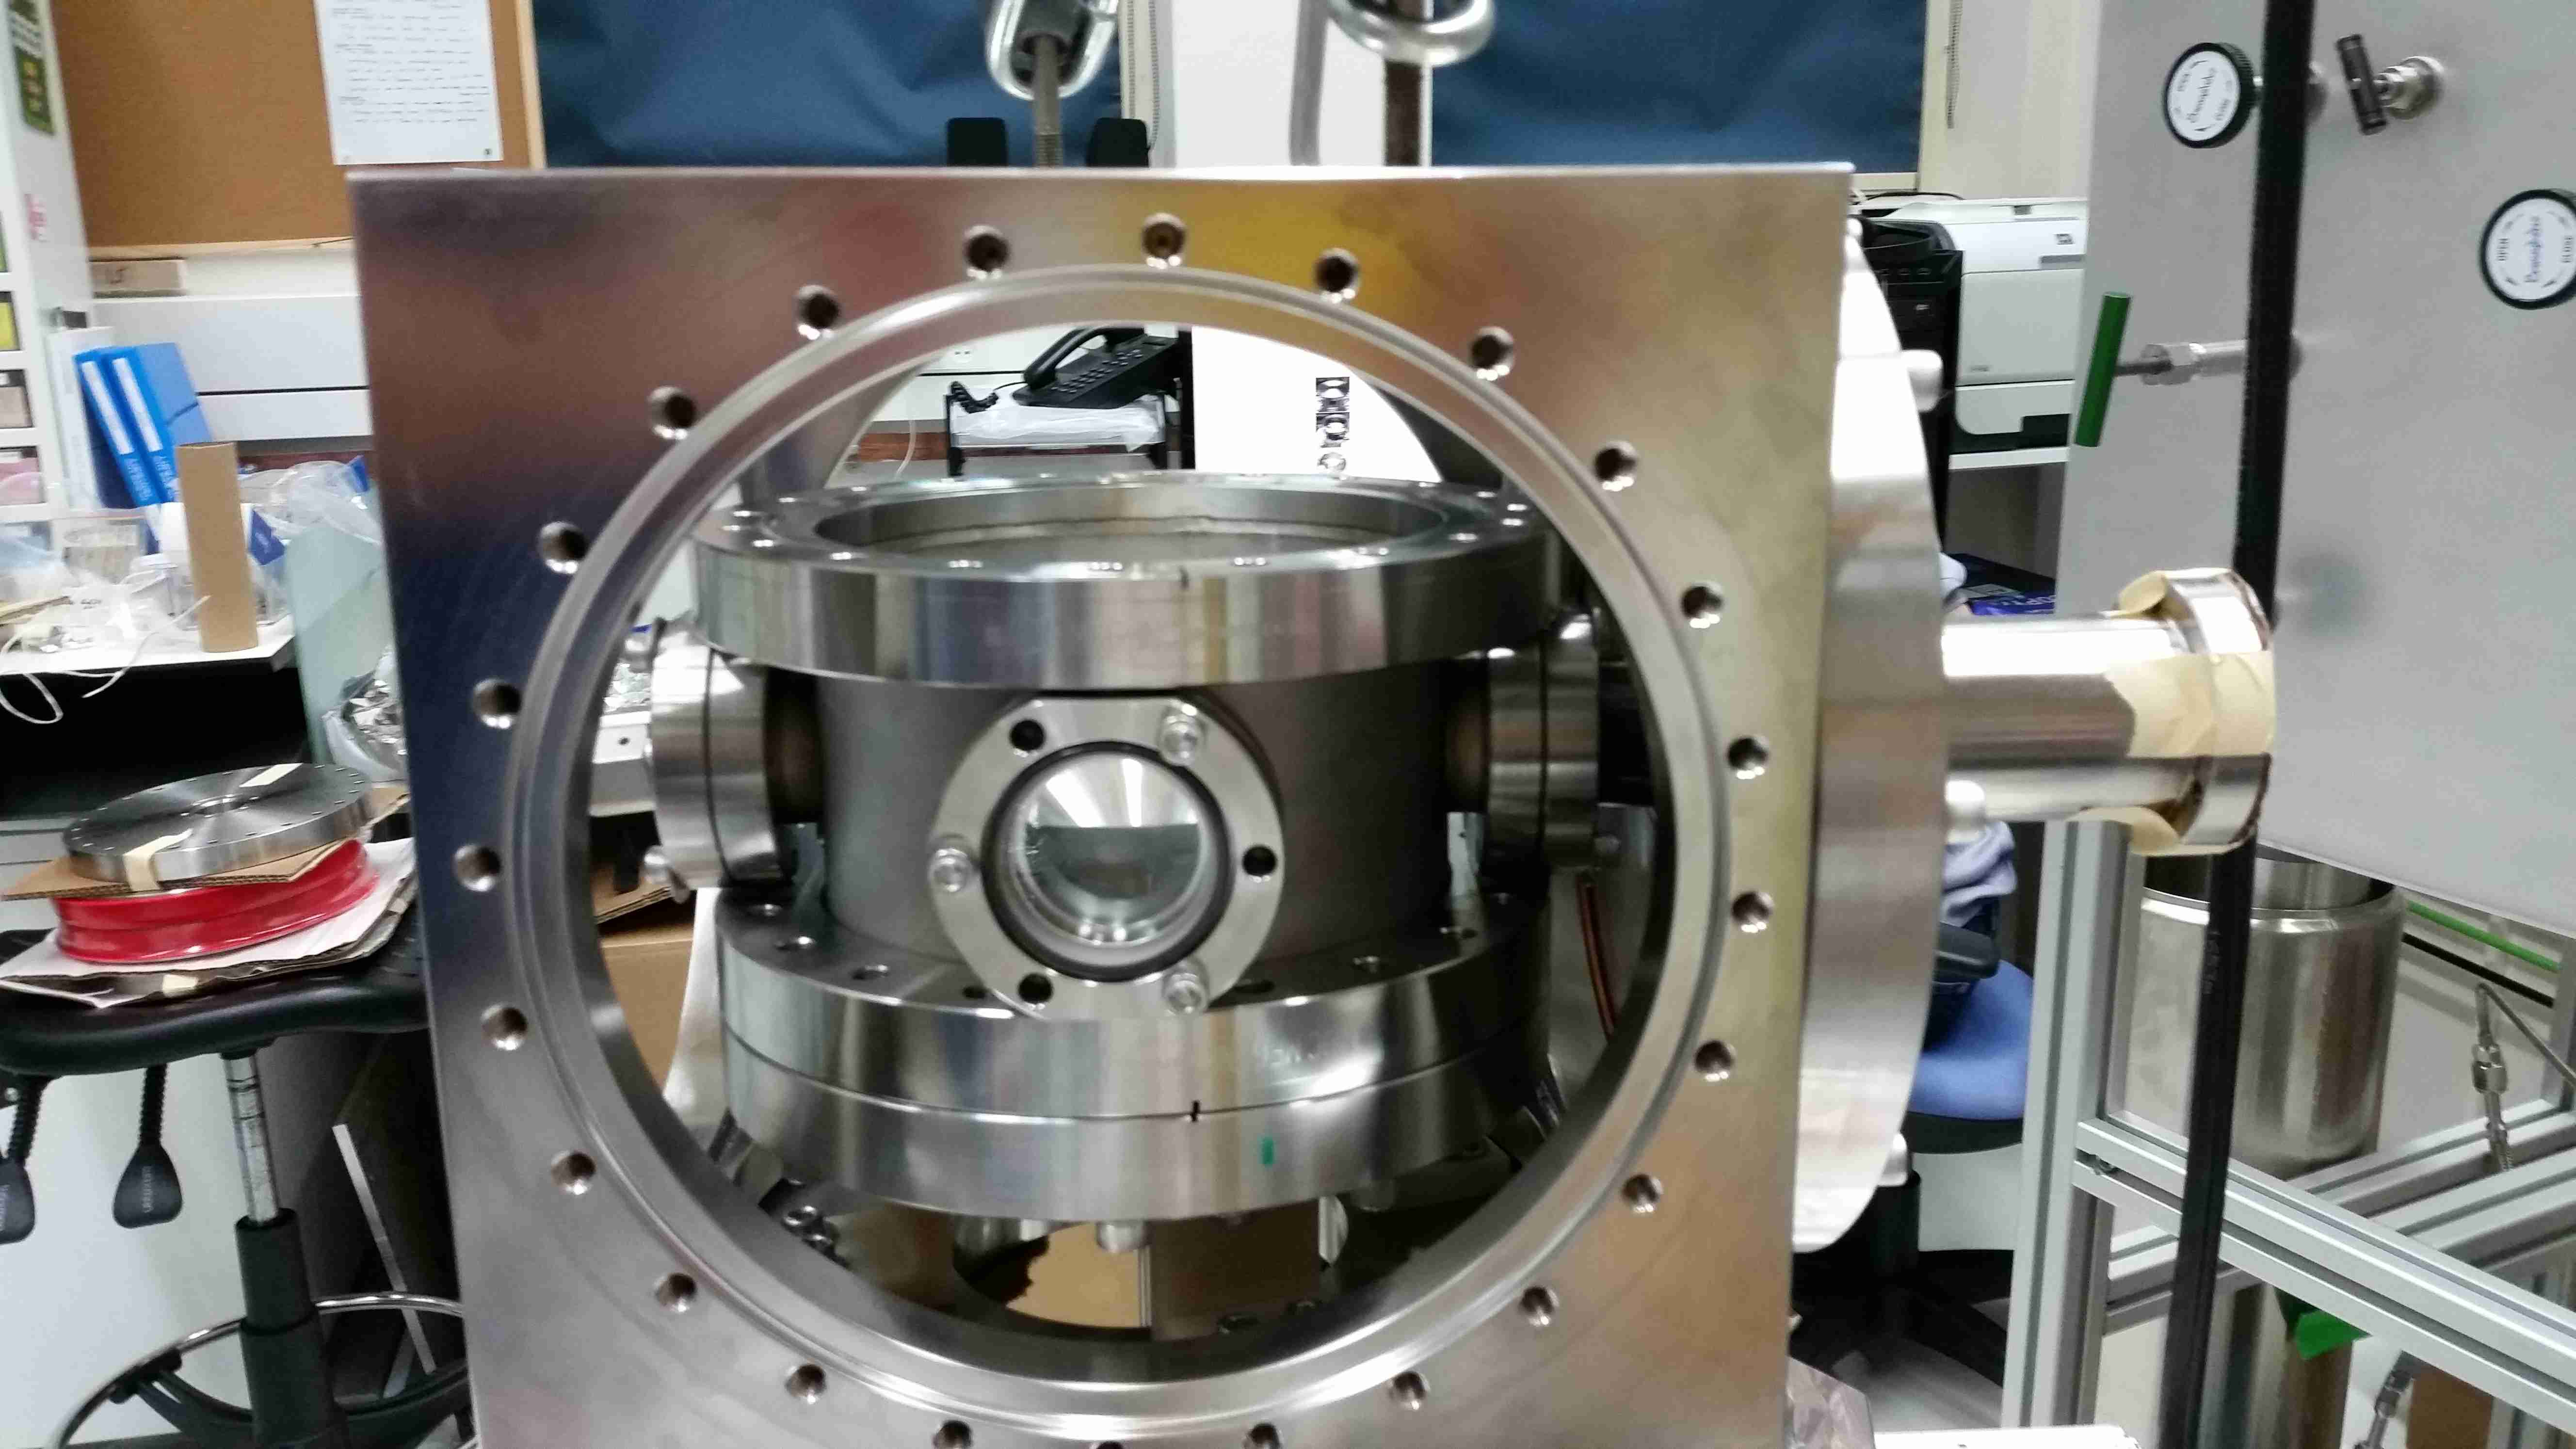
\includegraphics[width=\textwidth]{CryoOpen_small.jpg}
    \end{subfigure}
        \caption{(Top) CAD view of the cryogenic system. (Bottom) Pictue of the cryogenic system. \label{fig:cryo}}
\end{figure}


The OV is made of a 10" CF cube, with ports on all six faces (e.g., electrical feedthroughs, pumping ports, view ports, etc.). The space between the OV and IV is held constantly in vacuum for heat insulation. This vacuum is shared with the detector and with the heat exchanger chamber via 6" CF flexible bellows.

The IV is made of XXX~\,cm height cylinder with 6" CF flanges on the top and bottom parts of it, and it holds inside xenon. A XXX~" cold finger is welded to the top flange of the IV. The design of the cold finger is similar to the design of~\cite{xe100_instr2012}, the inner part of the cold finger is made of long fins, therefore the surface area of it is bigger resulting in a better heat transport. The upper part of the cold finger is in thermal contact with the cryo-cooler~\footnote{QDrive 20BB 9p6 A 3 AYNBNCO} via a cooper adapter. The copper adapter holds two $100\Omega$ pt resistor which are connected to a PID reader\footnote{cryo-con model 18i Cryogenic Temp Monitor} fot temperature measurements. A Cartridge-heater is also inserted to the copper adapter for emergency heating. 

The cryo-cooler provides up to 70 W of cooling power, and is connected via a 4 1/2" to 10" reducer to the OV from above, and reaching the IV top flange. Common cryo-coolers used for xenon experiments, work in maximal cooling mode permanently. The QDrive, instead, has temperature control allowing it vary the cooling power, which enables to set the temperature with fluctuations smaller then $0.1~\mathrm{C^{\circ}}$ on the cooler itself.

On the inner side of the bottom flange of the IV a thin SS funnel is installed collecting all LXe drops from the cold finger, and delivering them to the  detector part. This flange is connected to the detector part, via a 3 3/8" flexible bellows. This bellows hosts two small pipes (1/4") connected to the circulation system, and a third pipe coming from the funnel, all three pipes deliver LXe whereas the GXe is filling the bellows.

\subsection{The Detector Chamber}
\label{subsec:det}

The Detector chamber refers to the whole apparatus below the cryogenic system. It is built such that apart from the interface to the cryogenic system, it can be changed and modified easily for future experiments.
The interface unit is built out of 2 flanges welded together via 7 tubes, which serve as service ports for electrical and other feedthroughs. The upper flange, ISO-K 160, is part of the outer vessel and shares the insulation vacuum of the cryogenic system, the inner one , CF-8", is part of an inner vessel for future detectors, and would hold xenon inside. For our experiment we modified the CF flange to fit also a 4 1/2" CF flange which we use.

The OV is closed with a cylinder XXX~\,cm height closed from the bottom with another ISO-K 160 flange, the height of the cylinder is determined such that the maximal height of the whole apparatus is 190~\,cm, allowing the mobility of the detector through standard doors.
 
The 4 1/2" CF flange is connected to a closed vessel internally divided into two parts. This vessel serves as a xenon reservoir. The two parts of the vessel are connected to a spherical orb from above (inner part) and from below (outer part). LXe is circulated such that new LXe drips into the outer part and pumped from the inner one. This way the liquid level is controlled, and the sphere itself will always be filled with LXe. 

The main part of the detector is the spherical orb, which is made of fused silica. In the center of it, a smaller sphere is curved to hold the LXe, two invar pipes are connected to it from the top and bottom with SS mini-CF flanges at the end, to circulate the xenon (see Fig.~\ref{fig:sphere}). The sphere stands in the center of 20 PMTs\footnote{r8520-406 Hamamatsu 1" PMT} to detect light emitted from the LXe.

The bottom flange of the sphere is held using a brass holder to prevent force or torque applied on the sphere while mounting the detector. The brass holder is connected to a plate held from the top 8" flange, and is also used to allign this plate at first installation. 

The xenon sphere should be a large as possible however not too large to avoid double scatters. The fused silica sphere should be large enough in order to reduce internal reflections, but not too large to attenuate the scintillation light. The sphere is produced from HPFS 8655 Fused Silica. The refractive index of this material is 1.575 whereas of the LXe is 1.61, this prevents change in directionality when the light travels from the LXe to the fused silica. The measured transmittance of the HPFS is 99.75~\%cm, almost no light is absorbed in it.

The 20 PMTs are held with a special aluminum holder, coated with anti-reflection substance. The holder is made of two hemispheres hosting the PMTs in 3 rows all of them pointing to the center of the fused-silica sphere. the PMTs are held only via their bases. The bases are held using M2 PEEK screws. In Fig.~\ref{fig:detector} is a CAD and real view of the detector part.


The sources that will be used for exciting the xenon, and creating the supperradiance (signal) as well as the standard emission (background), will be $^{137} \mathrm{Cs}$ (662 keV) and $^{57} \mathrm{Co}$(122keV \& 136 keV) for ER and $^241$AmBe , D-D neutron generator, or neutron produced in an accelerator for NR . The mean free path for this energy is a couple of mm ($^{57} \mathrm{Co}$) and 0.5-3 cm ($^{137} Cs$), therefore a radius of 1cm was decided for the small sphere. For The large sphere GENAT4 simulation were used. Simulating 178nm photons randomly in the xenon and checking the ratio of detection. For the 99\% transmittance it is clear that the radius should be around 3 cm, see Fig.~\ref{fig:R2size}. 

\begin{figure}
	\centering
    \begin{subfigure}[b]{0.45\textwidth}
		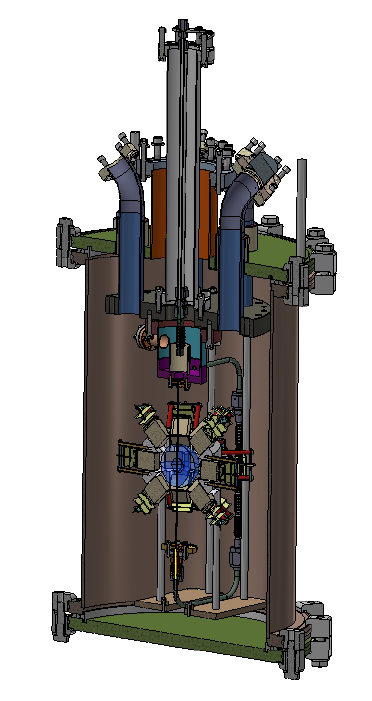
\includegraphics[width=0.75\textwidth , height=0.3\textheight]{detCAD.png}% Here is how to import 
	\end{subfigure}	
	\begin{subfigure}[b]{0.45\textwidth}
		\includegraphics[width=\textwidth , height=0.3\textheight]{DetChamber.JPG}% Here is how to import 
	\end{subfigure}	
		\caption{\label{fig:detector} (Left) CAD design of the detector part. (Right) The detector chamber open, in the middle is the PMT holder.}
	
\end{figure}
